
Relembrando, o objetivo deste trabalho é criar uma biblioteca no MATLAB que permita a resolução de problemas de otimização de trajetória de maneira facilitada, de forma que o usuário precise apenas modelar o problema, sem a necessidade de implementar a lógica da solução numérica. Para isso, é necessário que a biblioteca forneça uma interface de dados, de modo a permitir que o usuário entre com a modelagem do seu problema. Além disso, deve-se implementar a colocação trapezoidal como método de solução.

Para validação da implementação a ser realizada, o estudo de otimização de trajetória de subida de eVTOL em \cite{costa_otimizacao_2023}, o qual utiliza o software PSOPT citado na Seção \ref{sec:rev-bibliografica}, será replicado e os resultados serão comparados.


\section{Interface de Dados}
\label{sec:interface-dados}

Tendo como referência os softwares OptimTraj \cite{kelly_optimtraj_2022} e PSOPT \cite{becerra_psopt_2022}, a implementação será realizada utilizando \texttt{structures} como interface de dados. As duas principais serão:

\begin{itemize}
    \item \texttt{problem}: \texttt{structure} utilizada para entrar com o problema. Nela serão definidas as funções específicas do problema, as restrições, o palpite inicial de solução e informações adicionais, como número de fases e número de nós.
    \item \texttt{solution}: \texttt{structure} que conterá a solução do problema. Além dos valores do vetor solução - $\left[ t, \mathbf{x}, \mathbf{u} \right]^\intercal$ -, ela também conterá funções auxiliares usadas no seu cálculo e informações adicionais relacionadas a ele.
\end{itemize}

\begin{figure}[H]
    \centering
    \begin{subfigure}{0.48\linewidth}
    \centering
        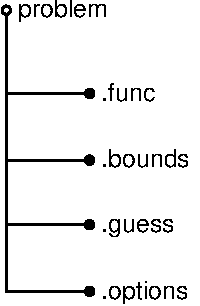
\includegraphics[width=0.4\textwidth]{Cap3/structures-problem.pdf}
        % \caption{Formato da \texttt{structure} \texttt{problem}}
    \end{subfigure}
    \hfill
    \begin{subfigure}{0.48\linewidth}
    \centering
        \includegraphics[width=0.4\textwidth]{Cap3/structures-solution.pdf}
        % \caption{Formato da \texttt{structure} \texttt{solution}}
    \end{subfigure}
    % 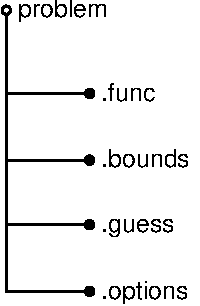
\includegraphics[width=0.4\textwidth]{Cap3/structures-problem.svg}
    \caption{Formatos das \texttt{structures} \texttt{problem} e \texttt{solution}}
    \label{fig:structures}
\end{figure}


% \section{Colocação Trapezoidal no MATLAB}
% \label{sec:colocação-trapezoidal}




\section{Trajetória de subida de eVTOL}
\label{sec:evtol}

O trabalho de referência considera um veículo multirrotor capaz de decolagem e pouso verticais, e visa encontrar a trajetória de subida que minimize o consumo energético da aeronave. Para modelar o problema, as variáveis de estado utilizadas foram

\begin{equation}
    \mathbf{x} = \left[
    \begin{aligned}
        s_x \\
        s_y \\
        v_x \\
        v_y \\
        E
    \end{aligned}
    \right],
\end{equation}

\noindent onde $[s_x, s_y]$ são as posições, $[v_x, v_y]$ as velocidades e $E$ a energia total da bateria utilizada. As variáveis de controle são os comandos de tração dos rotores

\begin{equation}
    \mathbf{u} = \left[
    \begin{aligned}
        T_x \\
        T_y
    \end{aligned}
    \right]
\end{equation}

\begin{figure}[H]
    \centering
    \includegraphics[width=0.72\textwidth]{Cap3/eVTOL.pdf}
    \caption{Diagrama de forças no eVTOL}
    \label{fig:evtol-forças}
\end{figure}

Conforme a figura \ref{fig:evtol-forças}, a dinâmica do sistema pode ser descrita como

\begin{equation}
\begin{aligned}
    m\ddot{p}_x &= F_x = T_x - D(\mathbf{v}) \cos(\gamma) - L(\mathbf{v}) \sin(\gamma) \\
    m\ddot{p}_y &= F_y = T_y - D(\mathbf{v}) \sin(\gamma) + L(\mathbf{v}) \cos(\gamma) - mg,
\end{aligned}
\end{equation}

\noindent de modo que as restrições diferenciais escrevem-se

\begin{equation}
\begin{aligned}
    \dot{s}_x &= v_x \\
    \dot{s}_y &= v_y \\
    \dot{v}_x &= \dfrac{1}{m} F_x \\
    \dot{v}_y &= \dfrac{1}{m} F_y,
\end{aligned}
\end{equation}

\begin{equation}
\begin{aligned}
    \dot{E}
    &= P_{total} \\
    &=
    \begin{aligned}
        &\left( 2 P_{ind,rotor,x} (1 + \chi) + T_x |\mathbf{v}| \cos(-\gamma) \right) \\
        &+ \left( 4 P_{ind,rotor,y} (1 + \chi) + T_y |\mathbf{v}| \sin(-\gamma) \right).
    \end{aligned}
\end{aligned}
\end{equation}

Para finalizar a formulação do PCO, dado que se almeja o consumo mínimo da bateria, define-se a função objetivo como

\begin{equation}
    J\left[ \mathbf{x} \left( t_f \right) \right] = E_f.
\end{equation}

\section{Movimento simples em uma dimensão}
\label{sec:movimento-simples}

\begin{equation}
    \mathbf{x} = \left[
        \begin{aligned}
            s_x \\
            v_x
        \end{aligned}
    \right]
\end{equation}

\begin{equation}
    \mathbf{u} = \left[
        \begin{aligned}
            F
        \end{aligned}
    \right]
\end{equation}

\begin{equation}
    \dot{\mathbf{x}} = \left[
        \begin{aligned}
            v \\
            F/m
        \end{aligned}
    \right]
\end{equation}

\begin{equation}
    J = \int_{t_0}^{t_f} \left[ F^2 \right] dt.
\end{equation}

\section{Braquistócrona}
\label{sec:braquistocrona}

\begin{equation}
    \mathbf{x} = \left[
        \begin{aligned}
            s_x \\
            s_y \\
            v
        \end{aligned}
    \right]
\end{equation}

\begin{equation}
    \mathbf{u} = \left[
        \begin{aligned}
            \theta
        \end{aligned}
    \right]
\end{equation}

\begin{equation}
    \dot{\mathbf{x}} = \left[
        \begin{aligned}
            v \cos(\theta) \\
            v \sin(\theta) \\
            -g \sin(\theta)
        \end{aligned}
    \right]
\end{equation}

\begin{equation}
    J = t_f.
\end{equation}

